\documentclass[tikz,border=4pt]{standalone}
\usepackage{tikz}
\usetikzlibrary{arrows.meta}
\definecolor{nebula}{HTML}{6366F1}
\definecolor{spark}{HTML}{14B8A6}
\begin{document}
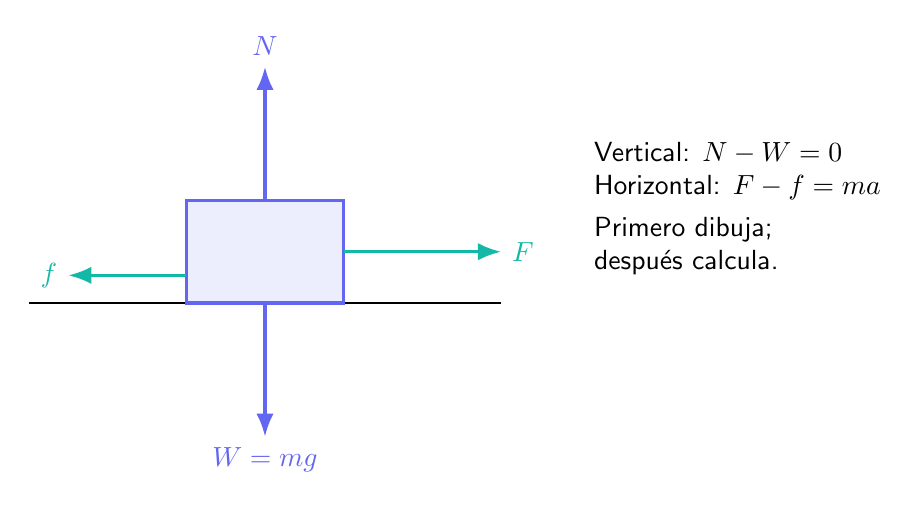
\begin{tikzpicture}[font=\sffamily,>=Latex]
  \draw[thick] (-3,0)--(3,0);
  \draw[fill=nebula!12,draw=nebula,very thick] (-1,0) rectangle (1,1.3);
  \draw[->,very thick,nebula] (0,1.3)--(0,3) node[above] {$N$};
  \draw[->,very thick,nebula] (0,0)--(0,-1.7) node[below] {$W=mg$};
  \draw[->,very thick,spark] (1,.65)--(3,.65) node[right] {$F$};
  \draw[->,very thick,spark] (-1,.35)--(-2.5,.35) node[left] {$f$};
  \node[align=left] at (6,1.2) {Vertical: $N-W=0$\\Horizontal: $F-f=ma$\\[3pt]Primero dibuja;\\despu\'es calcula.};
\end{tikzpicture}
\end{document}
